\documentclass[UTF8,a4paper,12pt,fontset=windows]{ctexart}

\usepackage{amsmath,amssymb,bm}
\usepackage{geometry}
\usepackage{booktabs,longtable,array,tabularx,multirow}
\usepackage{graphicx,float,caption}
\usepackage{xcolor,enumitem,fancyhdr}
\usepackage[hidelinks]{hyperref}

\geometry{left=2.5cm,right=2.5cm,top=2.5cm,bottom=2.4cm}
\setmainfont{Times New Roman}
\setCJKmainfont[BoldFont=SimHei]{SimSun}
\setCJKsansfont{SimHei}
\setlength{\parindent}{2em}
\setlength{\parskip}{0pt}
\linespread{1.28}
\setlist{nosep,leftmargin=2.2em}
\graphicspath{{../figures/}}
\captionsetup{font=small,labelsep=quad}
\pagestyle{fancy}
\fancyhf{}
\fancyhead[C]{烟幕干扰弹投放策略}
\fancyfoot[C]{\thepage}
\renewcommand{\headrulewidth}{0.4pt}
\setlength{\headheight}{15pt}
\renewcommand{\arraystretch}{1.18}
\newcommand{\R}{\mathbb{R}}
\newcommand{\meas}{\operatorname{meas}}
\newcommand{\clip}{\operatorname{clip}}
\newcolumntype{Y}{>{\raggedright\arraybackslash}X}
\newenvironment{algobox}[1]
  {\par\medskip\noindent\begin{minipage}{\textwidth}\small\hrule\medskip\textbf{#1}\par\medskip}
  {\medskip\hrule\end{minipage}\par\medskip}

\ctexset{
  section={format=\centering\heiti\zihao{3},beforeskip=1.0em,afterskip=0.7em},
  subsection={format=\heiti\zihao{4},beforeskip=0.8em,afterskip=0.5em},
  subsubsection={format=\heiti\zihao{-4},beforeskip=0.6em,afterskip=0.4em}
}

\begin{document}

\begin{center}
  {\heiti\zihao{2} 基于有限视线几何、连续事件与\\[0.2em]
  分层组合优化的烟幕干扰弹投放策略}
\end{center}

\begin{abstract}
针对多无人机投放烟幕干扰弹、以有限资源延长真目标有效遮蔽时间的问题，本文建立三维解析运动学、有限视线遮蔽和连续时间区间并集模型。题面未唯一规定“遮蔽目标”的几何口径，故以导弹至真目标圆柱几何中心的有限视线被烟幕球截断作为统一优化口径，并以圆柱内所有目标点的视线均被截断作为同策略的保守二次审计。求解过程采用“候选发现--连续验根--区间去重--独立复算”的证据链，避免把时间网格精度直接当作报告精度。

问题一按题定策略解析计算投放点、起爆点和运动轨迹，以均匀扫描隔离候选边界，再用 Brent 法连续验根。主口径有效区间为 $[8.0130,9.4481]$ s，时长 $1.4351$ s；完整圆柱审计时长为 $1.3916$ s。问题二对航向、速度、投放时刻和引信延时联合优化，差分进化产生全局候选后作连续局部精化，得到主口径遮蔽 $4.8325$ s；8 个独立种子均可行且终值差异仅处于机器精度量级。

问题三在同机固定航向、固定速度和投放间隔约束下，按新增并集长度组合三枚烟幕弹，本批最好可行方案形成连续区间 $[4.8077,11.4388]$ s，总时长 $6.6311$ s。问题四通过时间多样性候选池协调三架无人机，三个主要窗口互不重叠，总时长为 $15.7746$ s。问题五构造航路一致的同机投放包，再以有限状态搜索联合完成多机、多弹和多导弹指派；固定种子下得到经连续复算的可行解，总遮蔽为 $53.0839$ s，完整圆柱口径复核后为 $41.3551$ s。Q3 的种子离散不可忽略，Q5 尚未完成多种子审计，故均不作随机搜索稳定性强结论。

所有推荐方案均通过约束、连续边界和结果表回算检查。本文明确区分“已找到根的精度”和“扫描括区的完备性”：固定步长变号扫描仍可能漏掉极窄正区间或切触，因而不把机器精度残差解释为全局完备性证明；Q3--Q5 只陈述经验证的可行解，尤其不宣称 Q5 全局最优。

\par\noindent\textbf{关键词：烟幕干扰；有限视线；连续验根；区间并集；分层组合优化；保守审计}
\end{abstract}

\section{问题重述}

空地导弹以 $300$ m/s 沿初始位置至假目标原点的直线飞行。五架无人机在接到任务后可瞬时改变水平航向，随后以 $70\sim140$ m/s 等高度匀速直线飞行；同一架无人机的航向和速度保持不变。烟幕弹脱离无人机后作抛体运动，起爆后立即形成半径 $10$ m 的球形有效烟幕，球心以 $3$ m/s 下沉，单团烟幕的有效寿命为 $20$ s。真目标为下底面圆心 $(0,200,0)$、半径 $7$ m、高 $10$ m 的竖直圆柱\cite{problem}。

五个问题形成由确定性复算到连续优化、再到多资源组合的递进链：Q1 复算 FY1 给定单弹动作；Q2 优化 FY1 单弹；Q3 在 FY1 同一航路上协调三弹；Q4 令 FY1--FY3 各投一弹干扰 M1；Q5 令 FY1--FY5 每架至多投三弹，在 M1、M2、M3 之间分配资源。后三问还需填写可执行的投放点、起爆点和有效干扰时长。

\section{问题分析与技术路线}

\subsection{五问依赖与交付映射}

烟幕是否有效不是单纯的抛体落点问题，而是导弹、烟幕与目标三者随时间变化的几何事件。若按固定步长直接统计命中点，端点误差会进入目标函数；若把多弹单独时长相加，重叠区间又会被重复计分。因此本文将运动状态解析化，把时间网格限定为候选事件发现器，最终以连续根和区间并集定义目标。

\begin{table}[H]
\centering
\caption{五个子问题的输入、核心新增模块与向后接口}
\small
\begin{tabularx}{\textwidth}{cYYY}
\toprule
问题 & 输入与约束 & 本问新增模块 & 向后输出与检验重点\\
\midrule
Q1 & 题定航向、速度、投放和延时 & 有限视线、连续事件与双口径 & 几何判据、根区间和独立复算\\
Q2 & FY1 单弹四个连续决策量 & 有界非光滑连续优化 & 单弹候选、目标地形和多种子稳定性\\
Q3 & FY1 三弹共享航向与速度、间隔至少 1 s & 同航路候选包与区间去重 & 三弹组合、工作簿与重叠审计\\
Q4 & 三机各一弹 & 时间多样性候选池与跨机组合 & 互补时间窗和三机策略\\
Q5 & 五机至多十五弹、三枚来袭导弹 & 航路一致包、多机指派与有限状态搜索 & 三导弹并集、资源分配和可行性边界\\
\bottomrule
\end{tabularx}
\end{table}

\subsection{路线比较与选择理由}

运动学可直接用解析式表达，无需数值积分。真正的计算困难是有限视线的连续进入/退出，以及非光滑区间并集目标下的组合搜索。本文按“机理抽象--变量约束--数值求解--独立检验”的建模链组织五问\cite{modelbook}。表\ref{tab:route-comparison}比较可行路线。均匀计点法计算快，但会把步长误差混入时长；连续事件法保留计点法的候选发现能力，再用 Brent 法给端点，适合作为主计算。完整圆柱全遮蔽比中心视线严格、计算更贵，且题面语义并未指定它是唯一评分口径，因此只用于同方案保守审计。对于 Q3--Q5，一次性高维黑箱搜索不易保持同机航路和投放间隔，也难以审计；分层组合将领域结构先写入候选，再由有限状态搜索组合，计算代价和可行性都更可控\cite{nemhauser}。

\begin{table}[H]
\centering
\caption{候选路线的精度、代价与本文角色}
\label{tab:route-comparison}
\small
\begin{tabularx}{\textwidth}{p{2.5cm}YYY}
\toprule
路线 & 优点 & 主要风险 & 本文处理\\
\midrule
固定步长计点 & 实现简单、适合大量候选粗评 & 漏短区间；端点误差随步长变化 & 只作候选发现与快速基线，不作终稿报告值\\
中心有限视线连续事件 & 语义明确、代价低、可连续验根 & 是目标实体的代理口径 & 作为五问统一主口径，明确适用边界\\
完整圆柱全遮蔽 & 对实体目标更保守 & 连续最不利点搜索代价高，需括区完备性证据 & 同一策略的二次审计，不替代主目标\\
一次性全维黑箱优化 & 形式上统一 & 零平台、高维、约束修复和复现困难 & 不采用\\
候选--组合--连续复算 & 可显式保持航路和间隔，便于逐层核验 & 受路线库和保留宽度限制 & Q3--Q5 主路线，结论限定为已验证可行解\\
\bottomrule
\end{tabularx}
\end{table}

图\ref{fig:workflow}不再用抽象模块框代替物理过程，而以 Q1 的真实策略展示一次干扰事件：FY1 投放、烟幕弹起爆、云团下沉、首次进入视线管、最近点切换到导弹端点以及最终退出。右侧三个临界局部图对应式\eqref{eq:projection}的三种几何状态，底部事件带则把空间位置与连续根时刻逐一对齐。

\begin{figure}[H]
\centering
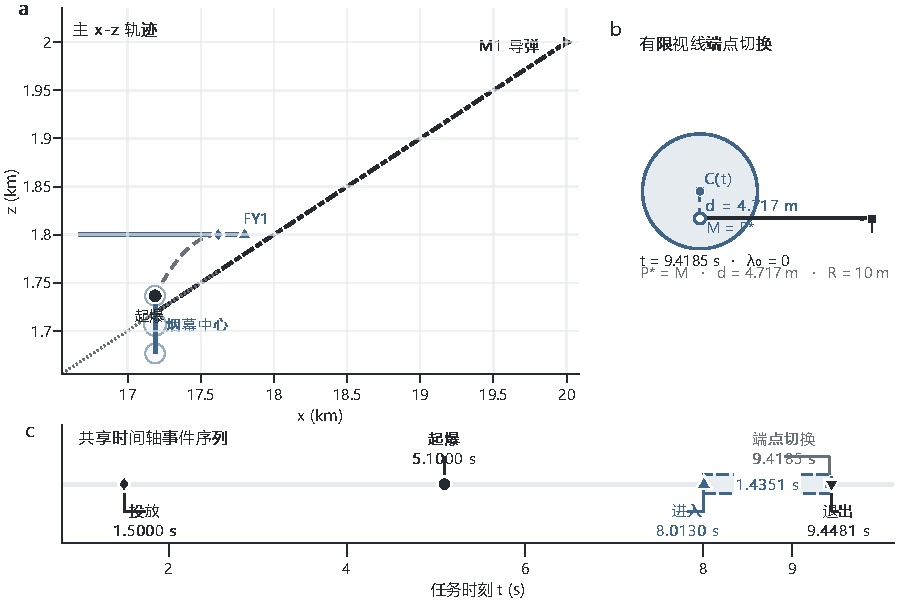
\includegraphics[width=0.98\textwidth]{modeling_workflow.pdf}
\caption{Q1 一次烟幕干扰的具体事件过程。A 给出 M1、FY1、投放点、起爆点和云团下沉轨迹；B--D 分别放大首次相切、最近点切至导弹端点和退出遮蔽；E 用同一时标连接投放、起爆、进入、端点切换和退出事件。全部时刻与坐标来自连续复算结果。}
\label{fig:workflow}
\end{figure}

\subsection{本文贡献与证据边界}

本文的工作重点不是堆叠算法名，而是保持三条闭环。第一，所有问题共享同一套运动和有限视线语义；第二，候选搜索与终稿连续复算分离，表格、图和摘要数字来自同一结果文件；第三，对中心视线、完整圆柱、时间离散和随机搜索分别给出其能证明与不能证明的内容。连续边界残差可以证明已括到的根求得准确，却不能单独证明扫描没有漏根；固定种子可证明复现，却不能单独证明全局最优。后文据此限制结论强度。

\section{模型假设、坐标系与符号说明}

\subsection{模型假设及其使用位置}

\begin{enumerate}
  \item 导弹在命中假目标前始终保持题面给定的直线匀速运动，不考虑末制导机动；该假设直接决定式\eqref{eq:missile-position}。
  \item 无人机转向时间忽略，转向后水平匀速且高度不变；同机所有烟幕弹继承同一水平初速度，并由结果表回算共享航向和速度。
  \item 烟幕弹只受重力作用，主计算取 $g=9.8$ m/s$^2$；不计空气阻力与风。另以 $g=9.81$ m/s$^2$ 做数值敏感性检查，但不把该检查扩展解释为风场鲁棒性。
  \item 起爆后的有效烟幕是半径恒为 $10$ m 的球体，在 $20$ s 内只发生球心匀速下沉；题面未给出的扩散、浓度衰减和风场不另行设参。
  \item 主评分采用真目标圆柱几何中心 $\bm q=(0,200,5)$ 的有限视线；完整圆柱全遮蔽只作二次审计，不反向替换主目标函数。
  \item 引信延时的数学可行域取 $\tau\geq0$。若工程上要求严格正延时，则另报告 $\tau=0.02$ s 的近边界方案。
\end{enumerate}

上述假设并非都已被现实数据验证。假设 1、2、4 来自题面理想化条件；假设 3 只做了重力常数复算；假设 5 通过双口径比较量化影响；风、定位和起爆时间联合扰动没有题面数据支持，故本文不编造其概率分布或 Monte Carlo 可靠度。

\subsection{主要符号}

\begin{table}[H]
\centering
\caption{主要符号、含义与单位}
\small
\begin{tabularx}{\textwidth}{p{3.0cm}Yp{2.0cm}}
\toprule
符号 & 含义 & 单位\\
\midrule
$\bm m_j^0,\bm m_j(t),T_j$ & 导弹 M$j$ 的初始位置、时刻 $t$ 的位置与撞击时刻 & m，s\\
$\bm u_i^0,\bm u_i(t)$ & 无人机 FY$i$ 的初始位置与时刻 $t$ 的位置 & m\\
$\theta_i,v_i,\bm h_i$ & 无人机水平航向角、速度和方向单位向量 & $^\circ$，m/s，--\\
$t_{ik}^{r},\tau_{ik},t_{ik}^{e}$ & 投放时刻、引信延时与起爆时刻 & s\\
$\bm p_{ik}^{r},\bm p_{ik}^{e}$ & 投放点与起爆点 & m\\
$\bm c_{ik}(t)$ & 起爆后烟幕球心位置 & m\\
$\bm q,\mathcal C$ & 真目标几何中心与圆柱实体 & m，--\\
$R_c,L_c,w_c,g$ & 烟幕半径、有效寿命、下沉速度与重力加速度 & m，s，m/s，m/s$^2$\\
$\lambda^*,d_{ikj},F_{ikj}$ & 有限线段投影系数、球心至视线距离与遮蔽裕度 & --，m，m\\
$I_{ikj},D_j$ & 单弹有效时间集合与导弹 $j$ 的遮蔽并集长度 & s，s\\
$a_{ikj}$ & 烟幕弹 $(i,k)$ 是否指派给导弹 $j$ & 0/1\\
\bottomrule
\end{tabularx}
\end{table}

\section{统一运动学与遮蔽几何模型}

\subsection{导弹、无人机与烟幕轨迹}

令假目标为坐标原点 $\bm o$。导弹 M$j$ 的速度向量和撞击时刻分别为
\begin{equation}
\bm v_j^m=300\frac{\bm o-\bm m_j^0}{\|\bm o-\bm m_j^0\|},\qquad
T_j=\frac{\|\bm o-\bm m_j^0\|}{300},
\label{eq:missile-velocity}
\end{equation}
故 $0\leq t\leq T_j$ 时
\begin{equation}
\bm m_j(t)=\bm m_j^0+\bm v_j^m t.
\label{eq:missile-position}
\end{equation}

无人机 FY$i$ 的水平单位方向记为 $\bm h_i=(\cos\theta_i,\sin\theta_i,0)$，则
\begin{equation}
\bm u_i(t)=\bm u_i^0+v_i\bm h_i t,\qquad 70\leq v_i\leq 140.
\label{eq:uav}
\end{equation}
第 $k$ 枚弹在 $t_{ik}^r$ 投放，延时 $\tau_{ik}$ 起爆，$t_{ik}^e=t_{ik}^r+\tau_{ik}$。投放点、起爆点与起爆后球心轨迹为
\begin{align}
\bm p_{ik}^r&=\bm u_i^0+v_i\bm h_i t_{ik}^r,\label{eq:release-point}\\
\bm p_{ik}^e&=\bm u_i^0+v_i\bm h_i t_{ik}^e-\frac12g\tau_{ik}^2\bm e_z,\label{eq:explosion-point}\\
\bm c_{ik}(t)&=\bm p_{ik}^e-w_c(t-t_{ik}^e)\bm e_z,
\quad t\in[t_{ik}^e,t_{ik}^e+L_c].
\label{eq:cloud}
\end{align}

\subsection{目标中心有限视线判据}

图\ref{fig:sightline-geometry}展示导弹、目标、烟幕球与有限视线段的真实语义。使用有限线段而非无限直线很重要：当垂足落在导弹之后或目标之后时，最近点应被截断到端点。

\begin{figure}[H]
\centering
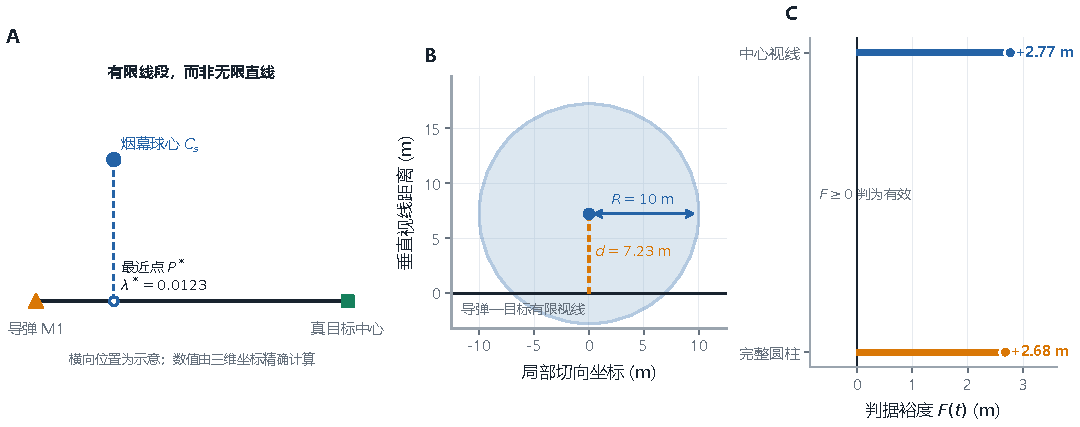
\includegraphics[width=0.98\textwidth]{finite_sightline_geometry.pdf}
\caption{有限视线判据的三层证据。A 为有限线段及最近点的非比例示意，B 为 $t=8.70$ s 的真实尺度局部截面，C 为同一时刻两种遮蔽口径的裕度复算；烟幕圆未被裁切。}
\label{fig:sightline-geometry}
\end{figure}

在时刻 $t$，记视线方向与烟幕相对向量分别为
\[
\bm s_j(t)=\bm q-\bm m_j(t),\qquad
\bm r_{ikj}(t)=\bm c_{ik}(t)-\bm m_j(t).
\]
导弹到目标中心的有限线段写为
\begin{equation}
\bm \ell_j(t,\lambda)=\bm m_j(t)+\lambda[\bm q-\bm m_j(t)],\qquad 0\leq\lambda\leq1.
\end{equation}
最近点来自一维凸二次函数
\begin{align}
\phi(\lambda)
&=\|\bm c_{ik}(t)-\bm\ell_j(t,\lambda)\|^2
=\|\bm r_{ikj}(t)-\lambda\bm s_j(t)\|^2,\label{eq:projection-objective}\\
\phi'(\lambda)
&=-2\bm s_j^{\mathsf T}\bm r_{ikj}+2\lambda\|\bm s_j\|^2.
\end{align}
对约束问题 $\min_{0\leq\lambda\leq1}\phi(\lambda)$，拉格朗日函数与 KKT 条件为
\begin{align}
\mathcal L&=\phi(\lambda)-\mu_0\lambda+\mu_1(\lambda-1),\\
2\|\bm s_j\|^2\lambda-2\bm s_j^{\mathsf T}\bm r_{ikj}-\mu_0+\mu_1&=0,
\quad \mu_0\lambda=0,
\quad \mu_1(1-\lambda)=0,
\quad \mu_0,\mu_1\geq0.
\end{align}
令 $\phi'(\lambda_0)=0$ 得到无限直线投影系数，由互补松弛可得分段解
\begin{align}
\lambda_0(t)&=\frac{\bm r_{ikj}^{\mathsf T}(t)\bm s_j(t)}{\|\bm s_j(t)\|^2},\\
\lambda^*(t)&=
\begin{cases}
0,&\lambda_0\leq0,\\
\lambda_0,&0<\lambda_0<1,\\
1,&\lambda_0\geq1,
\end{cases}
=\min\{1,\max\{0,\lambda_0(t)\}\}.
\label{eq:projection}
\end{align}
于是距离裕度与同号的平方裕度分别为
\begin{align}
d_{ikj}(t)&=\left\|\bm c_{ik}(t)-\bm\ell_j(t,\lambda^*)\right\|,
\qquad F_{ikj}(t)=R_c-d_{ikj}(t),\label{eq:margin}\\
G_{ikj}(t)&=R_c^2-d_{ikj}^2(t)
=F_{ikj}(t)\,[R_c+d_{ikj}(t)].\label{eq:squared-margin}
\end{align}
由于 $R_c+d_{ikj}(t)>0$，$F$ 与 $G$ 的符号及零点完全一致。将分段投影代回可得
\begin{equation}
G_{ikj}(t)=
\begin{cases}
R_c^2-\|\bm r_{ikj}\|^2,&\lambda_0\leq0,\\[2pt]
R_c^2-\|\bm r_{ikj}\|^2+\dfrac{(\bm r_{ikj}^{\mathsf T}\bm s_j)^2}{\|\bm s_j\|^2},&0<\lambda_0<1,\\[7pt]
R_c^2-\|\bm r_{ikj}-\bm s_j\|^2,&\lambda_0\geq1.
\end{cases}
\label{eq:squared-margin-piecewise}
\end{equation}
当烟幕有效、导弹尚未撞击且 $F_{ikj}(t)\geq0$ 时，判定主口径有效：
\begin{equation}
I_{ikj}=\{t\in[t_{ik}^e,\min(t_{ik}^e+L_c,T_j)]:F_{ikj}(t)\geq0\}.
\label{eq:interval}
\end{equation}

\subsection{完整圆柱保守审计及数值实现}

设真目标实体为 $\mathcal C$。若要求圆柱上每一点的视线均穿过烟幕球，则最不利距离为
\begin{equation}
d_{ikj}^{\rm cyl}(t)=\max_{\bm x\in\mathcal C}
\operatorname{dist}\bigl(\bm c_{ik}(t),[\bm m_j(t),\bm x]\bigr),
\label{eq:cylinder-distance}
\end{equation}
完整圆柱在时刻 $t$ 被遮蔽当且仅当 $d_{ikj}^{\rm cyl}(t)\leq R_c$。数值上将圆柱侧面、上底面和下底面分别参数化，以 96 个方位节点和 9 个线性节点发现候选极值区，再对候选区作有界连续精化。这一“离散括区--连续极值”过程用于减少全时域计算量\cite{prep}；96 个节点只是括区器，不被解释为最终方位精度。

独立交叉核验只在已验证的 Q2 完整圆柱方案的两个连续边界执行：把方位节点加密至 23040 个，密集采样最小余弦与连续极值结果的绝对差分别为 $7.77\times10^{-16}$ 和 $1.57\times10^{-14}$。该证据支持这两个边界处的方位极值，却不能替代对所有时刻、所有策略的全局完备性证明。因此完整圆柱值在全文中始终称为“保守二次审计”，不称为题意唯一真值。

\subsection{连续事件、区间并集与漏检边界}

在烟幕有效时间窗内以不超过 $0.01$ s 的步长扫描 $F_{ikj}(t)$，用来隔离符号变化区间；随后在每个括区上采用 Brent 法求连续根\cite{brent}，根绝对容差取 $10^{-12}$ s。对多枚烟幕弹，导弹 M$j$ 的总有效时长为
\begin{equation}
D_j=\meas\left(\bigcup_{i,k:a_{ikj}=1}I_{ikj}\right),
\label{eq:union}
\end{equation}
从而自动扣除同一导弹上的重叠时段。为把“连续根”转化为可审计的事件计算，首先定义单弹连续事件根集合
\begin{equation}
\mathcal E_{ikj}=
\left\{t\in[t_{ik}^e,\min(t_{ik}^e+L_c,T_j)]:G_{ikj}(t)=0\right\}.
\label{eq:event-root-set}
\end{equation}
对任一根 $e\in\mathcal E_{ikj}$，取足够小的 $\varepsilon>0$，由根两侧平方裕度的符号定义事件权重
\begin{equation}
\delta_{ikj}(e)=
\begin{cases}
+1,&G_{ikj}(e-\varepsilon)<0<G_{ikj}(e+\varepsilon),\\
-1,&G_{ikj}(e-\varepsilon)>0>G_{ikj}(e+\varepsilon),\\
0,&\text{切触且覆盖状态不改变}.
\end{cases}
\label{eq:event-weight}
\end{equation}
将有效区间统一写成半开区间 $[a,b)$；若多个事件同刻发生，先合并其净权重。把导弹 M$j$ 的全部事件时刻排序为
$e_{j,1}<e_{j,2}<\cdots<e_{j,M_j}$，并令 $\delta_{j,r}$ 为 $e_{j,r}$ 处的净权重，则
\begin{align}
n_j(t)&=\sum_{i,k}a_{ikj}\mathbf 1_{I_{ikj}}(t),\label{eq:coverage-count}\\
n_{j,0}&=0,\qquad n_{j,r}=n_{j,r-1}+\delta_{j,r},
\qquad n_j(t)=n_{j,r},\quad t\in[e_{j,r},e_{j,r+1}),\label{eq:event-count}\\
D_j&=\int \mathbf 1\{n_j(t)>0\}\,\mathrm dt
=\sum_{r=1}^{M_j-1}\mathbf 1\{n_{j,r}>0\}(e_{j,r+1}-e_{j,r}).\label{eq:event-union}
\end{align}
单弹时长之和超过并集的部分正是重复覆盖损失：
\begin{equation}
O_j=\sum_{i,k:a_{ikj}=1}\meas(I_{ikj})-D_j
=\int\bigl(n_j(t)-1\bigr)_+\,\mathrm dt.
\label{eq:overlap-loss}
\end{equation}
式\eqref{eq:event-root-set}--\eqref{eq:overlap-loss}给出“连续根--进入/退出--覆盖重数--区间并集”的完整事件链，也是后文具体事件图的直接数据来源。问题三、四最大化 $D_1$，问题五最大化
\begin{equation}
\max\;D_1+D_2+D_3.
\label{eq:q5-objective}
\end{equation}

需要区分两个误差层次。Brent 残差衡量“已经括到的根求得多准”；固定步长扫描决定“是否括到了所有根”。仅检测变号可能漏掉窄于扫描步长的正区间，也可能漏掉无变号切触。切触本身的测度可为 0，但它可能在参数扰动后生成短有效区间。本文已有 Q1 独立实现使用 $0.005$ s 扫描、192 个方位节点和 13 个线性节点复核；图\ref{fig:time-convergence}还比较均匀计点法相对连续验根的误差。现有证据足以支持报告区间的边界精度，但不构成对任意策略的漏根不可能性证明。

\subsection{共同约束与模型卡}

共同约束写为
\begin{equation}
\begin{aligned}
70\leq v_i\leq140,&\qquad t_{ik}^r\geq0,\qquad \tau_{ik}\geq0,
\qquad (\bm p_{ik}^e)_z\geq0,\\
t_{i,k+1}^{r}-t_{ik}^{r}&\geq1,\qquad
\sum_j a_{ikj}\leq1,\qquad a_{ikj}\in\{0,1\},\\
a_{ikj}=1&\Longrightarrow t_{ik}^e\leq T_j.
\end{aligned}
\label{eq:constraints}
\end{equation}
其中同机弹共享 $\theta_i,v_i$，且每架无人机最多使用三枚弹。最终方案不直接信任优化器内部变量，而是从导出的结果表重构投放点和起爆点，再逐项复算速度界、共享航路、投放间隔、起爆高度、指派和区间并集。

\section{问题一：给定策略的连续复算}

\subsection{目标、路线与形式化模型}

Q1 没有决策变量，目标是用题定策略计算 $I_{111}$ 及其测度。FY1 以 $120$ m/s 朝原点飞行，在 $1.5$ s 时投放，$3.6$ s 后起爆。运动状态由式\eqref{eq:release-point}--\eqref{eq:cloud}解析给出；目标中心和完整圆柱分别使用式\eqref{eq:interval}与式\eqref{eq:cylinder-distance}。

\subsection{算法披露}

\begin{algobox}{算法 1：给定策略的连续遮蔽区间复算}
\textbf{输入：}题定航向、速度、投放时刻、引信延时和导弹编号。\quad
\textbf{输出：}主口径与完整圆柱口径的有效区间、时长和边界残差。
\begin{enumerate}[label=\arabic*.,leftmargin=2em]
  \item 由解析式计算投放点、起爆点、导弹轨迹和烟幕球心轨迹；
  \item 在烟幕有效窗内扫描连续裕度，记录端点和符号变化括区；
  \item 对每个括区用 Brent 法求进入/退出根，并按中点符号重建正区间；
  \item 合并相邻区间，计算并集测度；
  \item 用第二几何实现和完整圆柱连续极值器复算，输出边界残差与约束违反量。
\end{enumerate}
\end{algobox}

\subsection{结果与机理解释}

由式\eqref{eq:release-point}--\eqref{eq:explosion-point}得到
\[
\bm p^r=(17620,0,1800)\ \text{m},\qquad
\bm p^e=(17188,0,1736.496)\ \text{m},\quad t^e=5.1\ \text{s}.
\]
连续验根给出目标中心视线有效区间 $[8.013006,9.448088]$ s，时长
\[
D_1=9.448088-8.013006=1.435082\ \text{s}.
\]
完整圆柱判据的进入时刻推迟至 $8.056445$ s，退出时刻基本不变，保守时长为 $1.391643$ s。图\ref{fig:q1-intervals}显示裕度曲线和有效区间：烟幕首先截断中心视线，随后才使圆柱最不利点的视线进入烟幕球，因此两种口径的差主要集中在进入边界。

\begin{figure}[H]
\centering
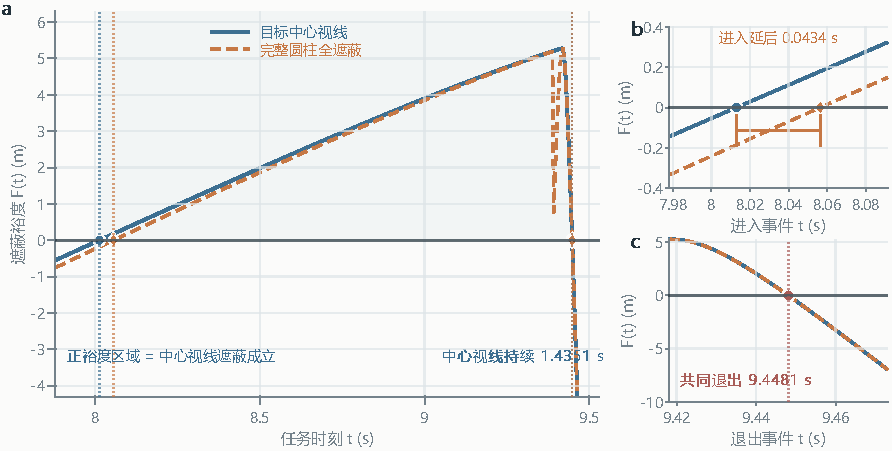
\includegraphics[width=0.96\textwidth]{q1_occlusion_intervals.pdf}
\caption{Q1 零点邻域的连续裕度与有效区间。A 聚焦进入、退出边界，B 直接标出完整圆柱口径的进入延迟 $0.0434$ s 及相应时长差。}
\label{fig:q1-intervals}
\end{figure}

\subsection{本问检验与小结}

主实现的最大边界距离残差为 $2.22\times10^{-11}$ m。独立实现采用 $0.005$ s 扫描、192 个方位节点、13 个线性节点和连续 Powell 表面精化，所得两种口径时长与主实现一致。把 $g$ 从 $9.8$ 改为 $9.81$ m/s$^2$ 后，中心视线时长变为 $1.448916$ s，变化 $0.013834$ s，占主结果的 $0.964\%$。这一复算只说明对两种常用重力常数的数值变化有限，不代表对风、定位或引信误差鲁棒。

\section{问题二：单机单弹连续优化}

\subsection{目标、路线与形式化模型}

决策向量为 $\bm x=(\theta,v,t^r,\tau)$，目标为
\begin{equation}
\max_{\bm x}\ D_1(\bm x)=\meas I_{111}(\bm x),
\quad -\pi\leq\theta\leq\pi,\quad 70\leq v\leq140,
\label{eq:q2-model}
\end{equation}
并满足式\eqref{eq:constraints}。实现时将变量改写为 $(\theta,v,t^e,\rho)$，其中 $t^e\in[0.03,14]$ s、$\rho\in[0,1]$、$\tau=\rho t^e$，从而自动保证 $0\leq\tau\leq t^e$ 和 $t^r=t^e-\tau\geq0$。

目标由若干区间长度组成，在区间出现或消失处不光滑，且大范围区域遮蔽时长为 0。图\ref{fig:q2-surface}的受控二维截面显示零平台和狭窄高值带，因此只用单初值局部优化存在明显风险。本文采用差分进化产生广域候选\cite{stornprice}，再以 Powell 无导数法和连续根精化\cite{powell,nocedal}。

\begin{figure}[H]
\centering
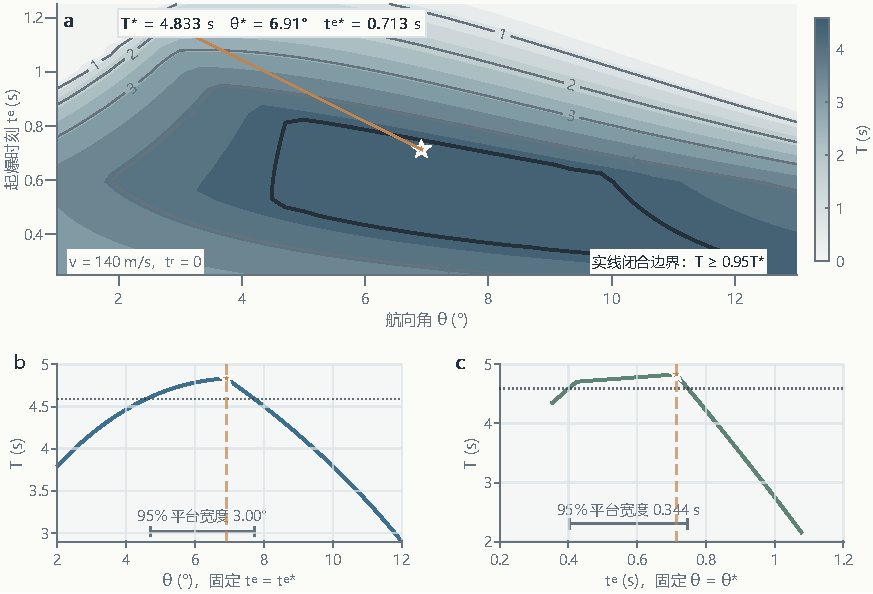
\includegraphics[width=0.96\textwidth]{q2_response_surface.pdf}
\caption{Q2 在速度 $140$ m/s、即时投放截面上的响应面与穿过连续解的两条正交剖面。主图仅保留关键等值线和 $95\%$ 高值边界，陶土色点为连续精化方案。}
\label{fig:q2-surface}
\end{figure}

\subsection{算法披露}

差分进化的种群倍率取 12，最大迭代 220 代，相对容差 $2\times10^{-6}$、绝对容差 $10^{-9}$；粗评分时间步长为 $0.01$ s，粗评分只用于排序。终稿策略一律重新计算连续边界和约束。多种子验证将种子从 20250808 连续取至 20250815，其余模型、边界和精化流程保持一致。

\begin{algobox}{算法 2：Q2 全局候选与连续精化}
\textbf{输入：}四维有界决策域、中心视线裕度函数和约束检查器。\quad
\textbf{输出：}连续复算后的可行单弹策略。
\begin{enumerate}[label=\arabic*.,leftmargin=2em]
  \item 差分进化在 $(\theta,v,t^e,\rho)$ 上搜索，以粗网格区间长度为主评分，并用极小的最大裕度引导项穿越零平台；
  \item 保留优良候选，转换为 $(\theta,v,t^r,\tau)$；
  \item 用无导数局部优化精化活动变量；
  \item 使用连续根重新计算区间，若约束违反非零则拒绝；
  \item 对 8 个独立种子重复上述过程，报告收敛缺口、可行率、计算代价和终值一致性，而非只报最好一次。
\end{enumerate}
\end{algobox}

\subsection{结果与边界语义}

表\ref{tab:q2}给出主口径方案。连续有效区间为 $[0.713246,5.545748]$ s，时长 $4.832502$ s。

\begin{table}[H]
\centering
\caption{Q2 目标中心视线口径的单弹策略}
\label{tab:q2}
\small
\begin{tabular}{ccccc}
\toprule
航向/$^\circ$ & 速度/(m/s) & $t^r$/s & $\tau$/s & 遮蔽时长/s\\
\midrule
6.9111 & 140.0000 & 0.0000 & 0.7132 & 4.8325\\
\bottomrule
\end{tabular}
\end{table}
对应空间位置为
\[
\bm p^r=(17800.000,0.000,1800.000)\ \text{m},\qquad
\bm p^e=(17899.129,12.015,1797.507)\ \text{m}.
\]

若把完整圆柱口径作为独立优化目标，闭可行域候选落在 $\tau=0$ 边界，保守时长为 $4.588064$ s。固定 $\tau=0.02$ s 后重新精化，得到 $4.588063$ s，仅损失 $1.96\times10^{-7}$ s。这里的两个圆柱值来自圆柱目标自身的优化，不能与主口径方案混成“同一策略前后变化”；跨问双口径图中将对此单独标注。

\subsection{本问检验与小结}

8 次全局搜索均可行，连续终值极差仅为 $3.3\times10^{-13}$ s，最大约束违反量为 0；其余搜索记账保留在验证文件，不在正文逐项列数。图\ref{fig:q2-multiseed}只保留与稳定性结论直接相关的 best-so-far 缺口、中位数和四分位带。结果说明在当前参数化和精化器下，8 个起点收敛到同一活动面；它仍不是解析的全局最优证书。

\begin{figure}[H]
\centering
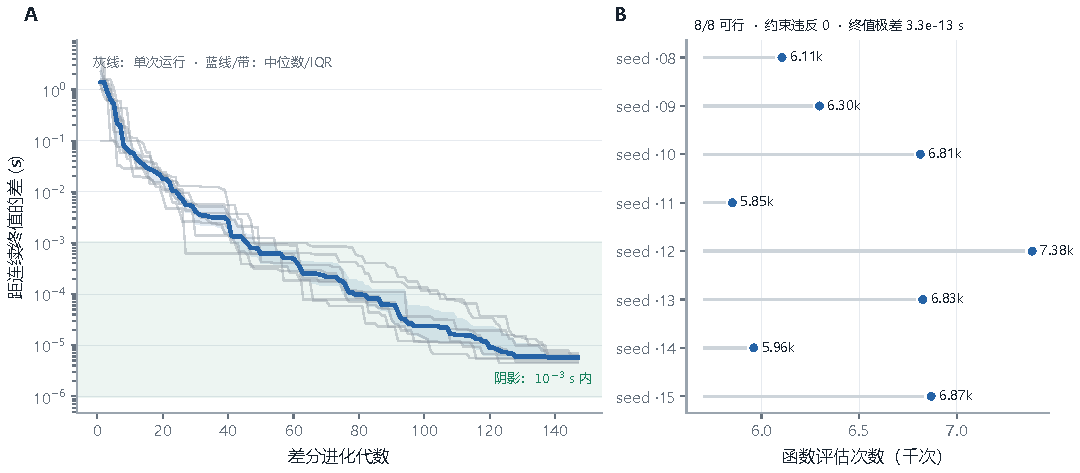
\includegraphics[width=0.96\textwidth]{q2_multiseed_stability.pdf}
\caption{Q2 八个独立随机种子的真实收敛缺口。灰线为单次 best-so-far 轨迹，蓝线与淡蓝带分别为中位数和 IQR；八次均可行，终值极差为 $3.3\times10^{-13}$ s。函数评估次数仅用于复现记账，不再作为正文图形。}
\label{fig:q2-multiseed}
\end{figure}

\section{问题三：FY1 三弹区间协同}

\subsection{目标、路线与形式化模型}

三枚弹共享 $\theta_1,v_1$，相邻投放至少间隔 1 s。若按单弹时长选前三枚，重叠窗口会被重复计分；因此形式化目标为
\begin{equation}
\max\ D_1=\meas(I_{111}\cup I_{121}\cup I_{131}),
\quad t_{1,k+1}^r-t_{1k}^r\geq1.
\label{eq:q3-model}
\end{equation}
为避免候选评分退化为单弹时长之和，令 $U_0=\varnothing$，第 $k$ 枚候选加入后的边际覆盖为
\begin{align}
\Delta_k&=\meas(I_{1k1}\setminus U_{k-1})
=\meas(I_{1k1})-\meas(I_{1k1}\cap U_{k-1})\notag\\
&=\meas(U_{k-1}\cup I_{1k1})-\meas(U_{k-1}),\label{eq:q3-marginal}\\
U_k&=U_{k-1}\cup I_{1k1},\qquad
\sum_{k=1}^{3}\Delta_k
=\sum_{k=1}^{3}[\meas(U_k)-\meas(U_{k-1})]
=\meas(U_3)=D_1.
\end{align}
上式是并集目标的望远镜分解。若 $U\subseteq V$，则
\begin{equation}
\meas(I\setminus U)\geq\meas(I\setminus V),
\label{eq:diminishing-return}
\end{equation}
即已有覆盖越多，同一候选的边际收益越小。因此重叠部分在第二次进入状态时边际收益为 0；搜索排序依据 $\Delta_k$，而不是 $\meas(I_{1k1})$。本问复用 Q2 的单弹连续区间函数，新增“同航路候选包”和“按新增并集长度计分”的组合层。

\subsection{算法披露}

路线、候选与保留包数量完整记录在验证文件。为避免把固定种子误当稳定性，种子 20250808--20250812 各独立运行一次；快速网格只负责候选排序，连续验根后的 $6.631110248$ s 才进入论文和结果表。

\begin{algobox}{算法 3：同航路三弹候选包搜索}
\begin{enumerate}[label=\arabic*.,leftmargin=2em]
  \item 枚举有限 $(\theta_1,v_1)$ 航路，生成能靠近 M1--目标视线的起爆候选；
  \item 在同一航路内按投放间隔构造至多三弹组合，使用新增并集长度而非单弹时长排序；
  \item 保留有限数量候选包，对其连续区间重新排序并局部精化；
  \item 导出工作簿后重构坐标、共享航向/速度、投放间隔和并集目标。
\end{enumerate}
\end{algobox}

\subsection{结果与解释}

\begin{table}[H]
\centering
\caption{Q3 FY1 三弹投放策略}
\label{tab:q3}
\scriptsize
\setlength{\tabcolsep}{3pt}
\begin{tabular}{ccccccccc}
\toprule
弹号 & 航向/$^\circ$ & $v$/(m/s) & $t^r$/s & $t^e$/s & 投放点 $(x,y,z)$/m & 起爆点 $(x,y,z)$/m & 单弹时长/s\\
\midrule
1 & 179.576 & 124.302 & 0.014 & 0.021 & $(17798.311,0.012,1800.000)$ & $(17797.414,0.019,1800.000)$ & 2.6043\\
2 & 179.576 & 124.302 & 1.880 & 5.900 & $(17566.298,1.729,1800.000)$ & $(17066.673,5.424,1720.831)$ & 2.5083\\
3 & 179.576 & 124.302 & 4.486 & 9.737 & $(17242.357,4.125,1800.000)$ & $(16589.672,8.953,1664.895)$ & 1.7015\\
\bottomrule
\end{tabular}
\end{table}

三枚弹的单独时长之和为 $6.814024$ s。合并后只有一个连续区间
\[
I_1=[4.807671,11.438782]\ \text{s},\qquad D_1=6.631110\ \text{s}.
\]
图\ref{fig:q3-union}把进入/退出根转换成事件轨和覆盖重数阶梯；其中 $n_1(t)>0$ 的区段构成并集，$n_1(t)\geq2$ 的区段为重复覆盖而非新增收益。

\begin{figure}[H]
\centering
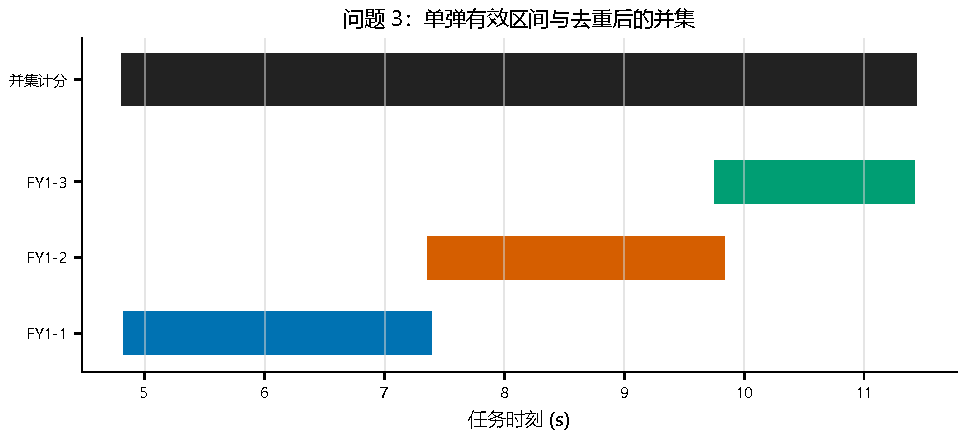
\includegraphics[width=0.96\textwidth]{q3_interval_union.pdf}
\caption{Q3 进入/退出根、单弹事件轨与覆盖重数。上层由连续根生成三条事件轨和去重并集；下层中 $n_1(t)\geq2$ 的区段累计为 $0.183$ s 重叠，故并集为 $6.631$ s。}
\label{fig:q3-union}
\end{figure}

\subsection{本问检验与小结}

相同策略按完整圆柱口径复核得到
\[
I_1^{\mathrm{cyl}}=[4.889896,7.411929]\cup[7.419477,11.438782]\ \text{s},
\qquad D_1^{\mathrm{cyl}}=6.541338\ \text{s},
\]
较主口径下降 $1.35\%$。三次投放满足至少 $1$ s 的间隔，并通过表\ref{tab:numerical-audit}的结果表回算。五个种子全部可行，但终值极差为 $0.9510$ s，离散不可忽略，说明该局部搜索仍受种子影响；本文采用本批最好且经连续复算的可行解，但不把它称为稳定或全局最优。收敛轨迹与终值分布见图\ref{fig:q34-multiseed}。

\section{问题四：三机单弹的时间互补}

\subsection{目标、路线与形式化模型}

三架无人机各投一弹。令 $\mathcal C_i$ 为第 $i$ 架无人机通过航路、落地和撞击时刻筛选后的可行单弹候选集，$I(c_i)$ 为候选 $c_i$ 的连续有效区间，则目标为
\begin{equation}
\max_{c_i\in\mathcal C_i\ (i=1,2,3)}
D_1(c_1,c_2,c_3)
=\meas\!\left(I(c_1)\cup I(c_2)\cup I(c_3)\right).
\label{eq:q4-model}
\end{equation}
三机初始位置差异显著。若分别选择各自单弹最大值，三个窗口可能重叠；本问先按有效区间的时间中心构造早、中、晚多样性候选池，再以跨机并集评分组合。

\subsection{算法披露}

航路与候选规模完整记录在验证文件；正文只保留影响结论的证据。种子 20250808--20250812 各独立运行一次，快速计点只用于粗筛，终稿连续复算值为 $15.774625$ s。两种评分口径不同，故不把粗值与连续值之差解释为真实性能变化。

\subsection{结果与解释}

\begin{table}[H]
\centering
\caption{Q4 FY1--FY3 联合策略}
\label{tab:q4}
\scriptsize
\setlength{\tabcolsep}{3pt}
\begin{tabular}{ccccccccc}
\toprule
无人机 & 航向/$^\circ$ & $v$/(m/s) & $t^r$/s & $t^e$/s & 投放点 $(x,y,z)$/m & 起爆点 $(x,y,z)$/m & 单弹时长/s\\
\midrule
FY1 & 5 & 110 & 0.962 & 1.088 & $(17905.438,9.225,1800.000)$ & $(17919.170,10.426,1799.923)$ & 4.7919\\
FY2 & 255 & 140 & 3.145 & 9.938 & $(11886.037,974.684,1400.000)$ & $(11639.918,56.156,1173.933)$ & 5.0713\\
FY3 & 145.032 & 140 & 28.889 & 39.370 & $(2685.732,-682.088,700.000)$ & $(1483.177,158.948,161.630)$ & 5.9115\\
\bottomrule
\end{tabular}
\end{table}

主口径三个区间分别为
\begin{equation*}
\begin{aligned}
I_1&=[1.227985,6.019839]\ \text{s},\\
I_2&=[10.195554,15.266823]\ \text{s},\\
I_3&=[39.517183,45.428685]\ \text{s}.
\end{aligned}
\end{equation*}
一般地，若按进入时刻排序后 $I_r=[\alpha_r,\beta_r]$ 且
\begin{equation}
\beta_r<\alpha_{r+1}\quad(r=1,2),
\end{equation}
则覆盖重数在每个退出事件后回到 0，故
\begin{equation}
D_1=\sum_{r=1}^{3}(\beta_r-\alpha_r),\qquad
g_r=\alpha_{r+1}-\beta_r>0.
\label{eq:q4-gaps}
\end{equation}
本方案两段空窗分别由 $g_1,g_2$ 给出，三者互不重叠，总时长等于三个单弹时长之和，为 $15.774625$ s。图\ref{fig:q4-synergy}以三条“投放--起爆--进入--退出”动作链和覆盖状态节点显示两个接力空窗，而不是把“各自最长”当作“并集最长”。

\begin{figure}[H]
\centering
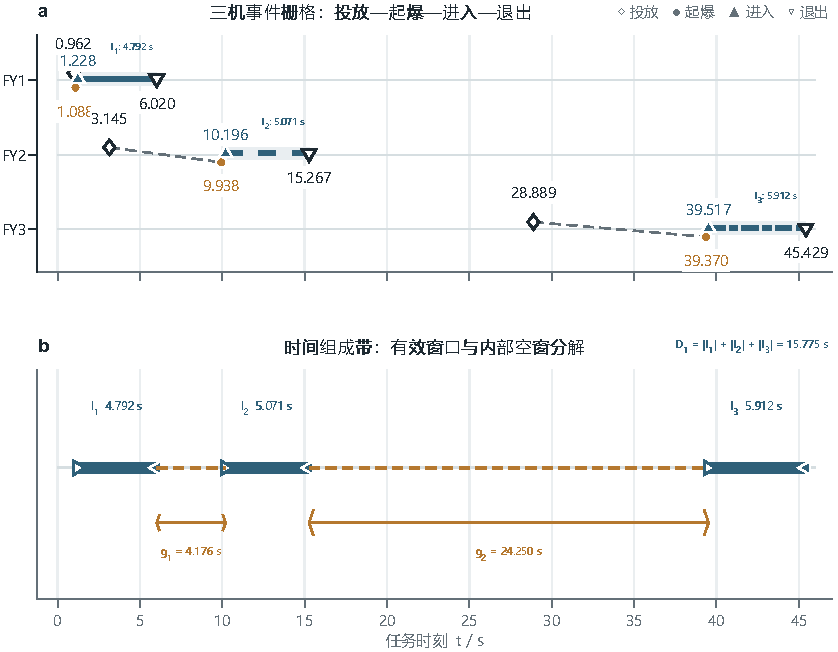
\includegraphics[width=0.96\textwidth]{q4_temporal_synergy.pdf}
\caption{Q4 三架无人机的动作链与覆盖状态接力。圆形状态节点表示 $n(t)=1$ 的有效窗口，节点间箭头表示 $n(t)=0$ 的两个内部空窗；三个主窗口互不重叠，故联合目标等于三段时长之和。}
\label{fig:q4-synergy}
\end{figure}

\subsection{本问检验与小结}

完整圆柱复核后总时长为 $10.430630$ s，下降 $33.88\%$。这一变化明显大于 Q3，原因是 FY3 的后期烟幕靠近地面，目标圆柱上下边缘对应的最不利视线更难同时进入半径 $10$ m 的烟幕球。方案通过表\ref{tab:numerical-audit}的结果表回算；五个种子全部可行，终值极差为 $38$ ms。图\ref{fig:q34-multiseed}显示多数种子停在同一平台，仅一个种子取得小幅改进，因此仍没有全局最优证明。

\begin{figure}[H]
\centering
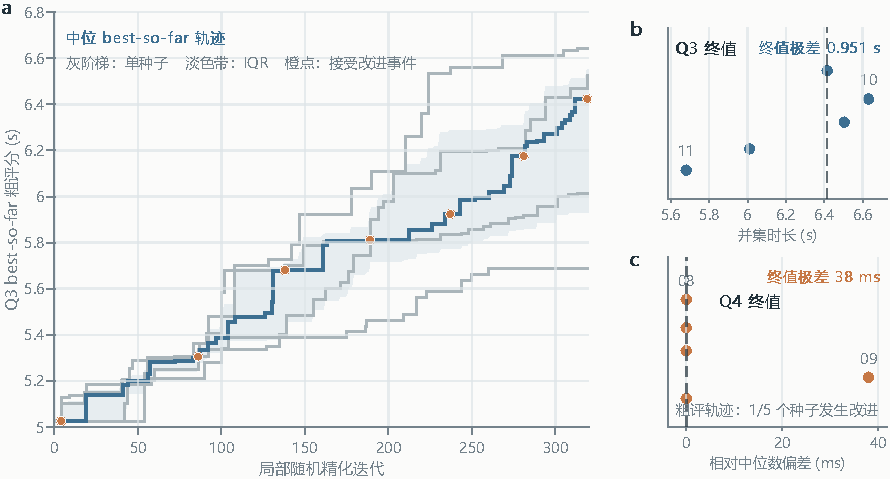
\includegraphics[width=0.98\textwidth]{q3_q4_multiseed_stability.pdf}
\caption{Q3、Q4 五个独立种子的事件阶梯与连续终值脊线。左侧按 best-so-far 事件前向保持，不用直线插值虚构改进；右侧只标端点极差和极端种子。}
\label{fig:q34-multiseed}
\end{figure}

\section{问题五：五机多弹多目标分层优化}

\subsection{目标、路线与形式化模型}

Q5 同时含连续航路、连续时序和离散指派。设 $a_{ikj}=1$ 表示弹 $(i,k)$ 指派给导弹 $j$，则目标为式\eqref{eq:q5-objective}，并满足式\eqref{eq:constraints}、同机共享 $\theta_i,v_i$ 以及每机至多三弹。官方结果表为每枚弹提供单一“干扰的导弹编号”，故模型使用 $\sum_j a_{ikj}\leq1$；不同导弹在同一绝对时刻被遮蔽可分别计入，不同烟幕弹对同一导弹的重叠只计一次。

直接在全部连续变量和 0--1 指派上做一次性黑箱优化，维数高且难以维持航路一致性。本文先用平面共线条件生成可能靠近导弹--目标视线的起爆时刻，再构造同机航路一致包，最后用有限状态搜索联合指派。

为使搜索状态与原优化问题严格对应，令 $\mathcal R_i$ 为无人机 $i$ 的候选航路集，$y_{ir}$ 表示是否锁定航路 $r$；令 $\mathcal C_i$ 为该机在各航路上生成的候选弹集，$x_{cj}$ 表示候选弹 $c$ 是否指派给导弹 $j$。记 $i(c),r(c),t_c^r$ 分别为候选的无人机、航路和投放时刻，则离散组合层写为
\begin{equation}
\max_{x,y}\quad
\sum_{j=1}^{3}
\meas\!\left(\bigcup_{c:x_{cj}=1}I_{cj}\right),
\label{eq:q5-route-model}
\end{equation}
满足
\begin{equation}
\begin{aligned}
&\sum_{r\in\mathcal R_i}y_{ir}\leq1,
&&i=1,\ldots,5,\\
&x_{cj}\leq y_{i(c),r(c)},
&&c\in\mathcal C_{i(c)},\\
&\sum_{c:i(c)=i}\sum_{j=1}^{3}x_{cj}\leq3,
&&i=1,\ldots,5,\\
&\sum_{j=1}^{3}x_{cj}\leq1,
&&c\in\bigcup_i\mathcal C_i,\\
&x_{cj}+x_{d\ell}\leq1,
&&i(c)=i(d),\ |t_c^r-t_d^r|<1,\\
&x_{cj},y_{ir}\in\{0,1\}.&&
\end{aligned}
\label{eq:q5-route-constraints}
\end{equation}
式\eqref{eq:q5-route-constraints}依次强制单航路、路线--候选联动、每机至多三弹、单弹单目标和至少 $1$ s 的投放间隔；连续可行性已在生成 $\mathcal C_i$ 时筛除。

把已选路线包的状态写为
\begin{equation}
\mathcal S=\bigl(\mathcal U_1,\mathcal U_2,\mathcal U_3;
\rho_1,\ldots,\rho_5;
b_1,\ldots,b_5;
t^{r,\mathrm{last}}_1,\ldots,t^{r,\mathrm{last}}_5\bigr),
\label{eq:q5-state}
\end{equation}
其中 $\mathcal U_j$ 是导弹 $j$ 已形成的区间并集，$\rho_i$ 是无人机 $i$ 已锁定的航路参数，$b_i\leq3$ 是该机已用弹数。候选弹 $c=(i,k,j,I_c)$ 只有在共享航路、投放间隔、剩余弹数和起爆约束均满足时才允许转移；其真实增量不是单弹时长，而是
\begin{align}
\Delta J(c\mid\mathcal S)
&=\meas(\mathcal U_j\cup I_c)-\meas(\mathcal U_j)
=\meas(I_c\setminus\mathcal U_j),\label{eq:q5-transition}\\
\mathcal U_j'&=\mathcal U_j\cup I_c,\qquad
b_i'=b_i+1,\qquad t_i^{r,\mathrm{last}\prime}=t_c^r,\notag\\
J(\mathcal S')&=J(\mathcal S)+\Delta J(c\mid\mathcal S).
\end{align}
式\eqref{eq:q5-transition}同时处理同弹不同目标的离散指派和同目标多弹的连续重叠；因此有限状态搜索的每次扩展都与最终连续并集目标一致。

\subsection{算法披露与质量标定}

路线、候选和保留包规模写入验证文件，不在正文逐项列数。固定种子 20250808 下，入选状态经连续复算为 $53.083939170$ s。路线库仍是有限的，且本问尚未完成多种子重复，因此该流程只提供一组可复现且经连续复算的可行解，没有给出搜索稳定性、松弛上界或全局最优性间隙。

\begin{algobox}{算法 4：Q5 航路一致包与多机指派搜索}
\textbf{输入：}五架无人机、三枚导弹、候选航路库、每机至多三弹约束。\quad
\textbf{输出：}经连续复算且可写入结果表的多机策略。
\begin{enumerate}[label=\arabic*.,leftmargin=2em]
  \item 对每条 $(\theta_i,v_i)$ 航路，利用视线平面共线关系生成候选起爆时刻，反求延时和投放时刻；
  \item 删除起爆地下、撞击后起爆、非正遮蔽和其他不可行候选；
  \item 在同一航路内构造至多三弹的路线包，强制共享航向、速度和投放间隔；
  \item 在五机之间用有限状态搜索联合选择路线包和导弹指派，以新增并集长度更新状态；
  \item 对保留状态逐弹连续验根，重新合并三枚导弹的区间；
  \item 从最终工作簿重构全部坐标和约束，只有最大违反量为 0 的方案进入论文。
\end{enumerate}
\end{algobox}

Q3--Q5 的候选数、航路数和保留包数只作为复现记账写入验证文件，不再单独绘成正文统计图。快速评分负责筛选，式\eqref{eq:event-union}的连续复算值负责报告；两者口径不同，不能据其差值计算严格改进率或最优性间隙。

\subsection{推荐策略及空间解释}

表\ref{tab:q5-strategy}列出 15 枚烟幕弹的主要时序决策，完整投放点和起爆点已写入题目要求的结果表。每架无人机恰使用三枚弹，这是当前可行解的资源使用结果，不意味着未知全局最优解必然用满全部烟幕弹。

\begingroup
\scriptsize
\setlength{\tabcolsep}{5pt}
\begin{longtable}{ccccccc}
\caption{Q5 固定种子受限搜索得到的经验证可行投放策略}\label{tab:q5-strategy}\\
\toprule
无人机 & $\theta/^\circ$ & $v$/(m/s) & 弹$\to$目标 & $t^r$/s & $t^e$/s & 单弹时长/s\\
\midrule
\endfirsthead
\multicolumn{7}{c}{续表\thetable}\\
\toprule
无人机 & $\theta/^\circ$ & $v$/(m/s) & 弹$\to$目标 & $t^r$/s & $t^e$/s & 单弹时长/s\\
\midrule
\endhead
\midrule
\multicolumn{7}{r}{续下页}\\
\endfoot
\bottomrule
\endlastfoot
FY1&180&130&1$\to$M1&0.104&3.063&2.3092\\
FY1&180&130&2$\to$M1&2.676&7.313&2.2692\\
FY1&180&130&3$\to$M1&5.156&10.813&1.2996\\
FY2&250&110&1$\to$M2&5.045&9.563&4.6893\\
FY2&250&110&2$\to$M1&6.063&13.063&4.8458\\
FY2&250&110&3$\to$M3&10.766&17.063&3.7620\\
FY3&130&130&1$\to$M3&22.029&30.063&4.4498\\
FY3&130&130&2$\to$M1&23.046&31.313&4.8297\\
FY3&130&130&3$\to$M2&24.294&32.313&4.4988\\
FY4&230&140&1$\to$M2&3.170&15.313&4.5449\\
FY4&230&140&2$\to$M1&4.880&18.063&4.7915\\
FY4&230&140&3$\to$M3&8.348&21.313&3.2456\\
FY5&120&130&1$\to$M3&12.406&14.313&3.8861\\
FY5&120&130&2$\to$M1&13.517&17.813&2.9813\\
FY5&120&130&3$\to$M2&19.977&21.063&2.6383\\
\end{longtable}
\endgroup

图\ref{fig:q5-xy}显示投放点和起爆点的平面关系。同一架无人机的水平位移方向一致，是共享航向、共享速度约束的直接几何结果；图只用于平面解释，完整三维坐标仍以结果表为准。

\begin{figure}[H]
\centering
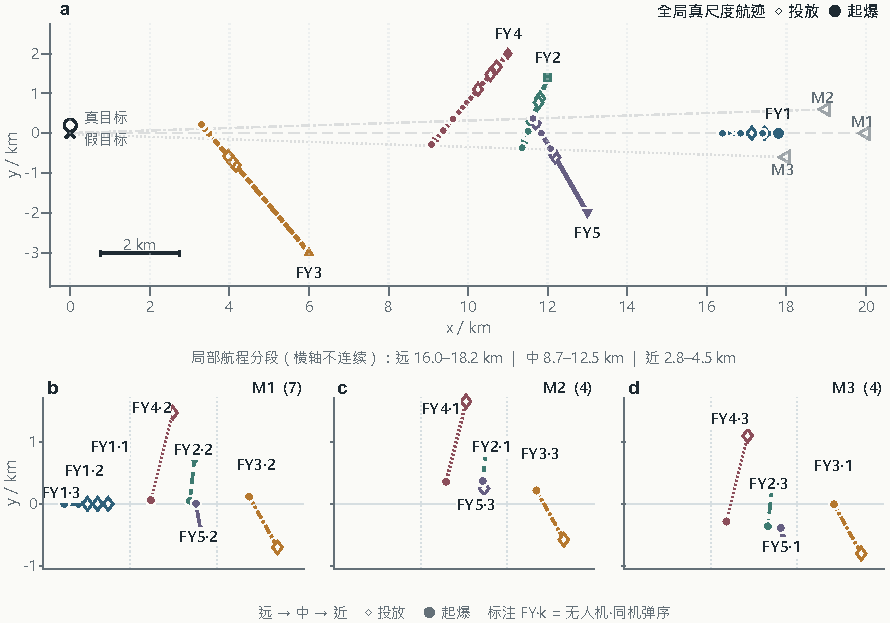
\includegraphics[width=0.98\textwidth]{q5_xy_strategy.pdf}
\caption{Q5 空间策略的全局真比例主图与 M1--M3 分段局部镜头。颜色只表示无人机，分面表示导弹，空心菱形和实心圆分别表示投放与起爆事件。}
\label{fig:q5-xy}
\end{figure}

\subsection{遮蔽并集结果与解释}

\begin{table}[H]
\centering
\caption{Q5 按导弹汇总的遮蔽时长}
\label{tab:q5-duration}
\begin{tabular}{cccc}
\toprule
导弹 & 目标中心视线/s & 完整圆柱审计/s & 审计下降率/\%\\
\midrule
M1 & 22.9078 & 17.9772 & 21.52\\
M2 & 16.3713 & 12.1515 & 25.78\\
M3 & 13.8049 & 11.2263 & 18.68\\
\midrule
合计 & 53.0839 & 41.3551 & 22.09\\
\bottomrule
\end{tabular}
\end{table}

主口径总目标为 $53.083939$ s。这个总时长是三枚导弹各自并集长度之和；图\ref{fig:q5-gantt}以逐弹进入--退出事件弧及覆盖数阶梯展示合并关系。M1 的覆盖由多个时间段串联，M2、M3 仍有空档，因而该图同时给出继续搜索可能利用的位置，也说明当前结果不是上界。

\begin{figure}[H]
\centering
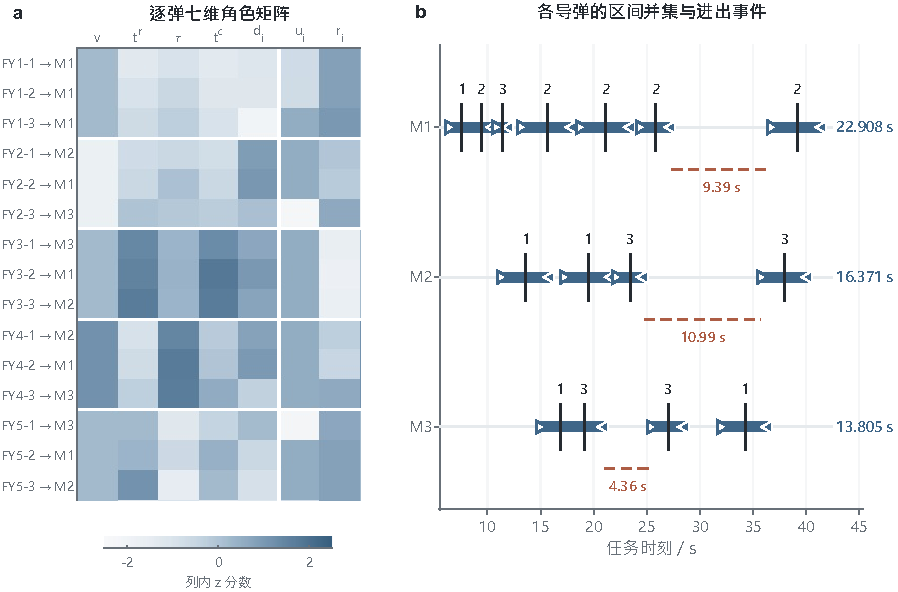
\includegraphics[width=0.98\textwidth]{q5_coverage_gantt.pdf}
\caption{Q5 十五枚烟幕弹按导弹分组的进入--退出事件弧与覆盖数阶梯 $n_j(t)$。三角事件节点和浅弧标识单弹进入、退出配对，阶梯由全部事件扫描得到，双向箭头标出每枚导弹的最大内部空窗。}
\label{fig:q5-gantt}
\end{figure}

\subsection{本问检验与小结}

相同决策按完整圆柱口径复核后，三枚导弹的并集均低于中心视线结果。图\ref{fig:criterion-sensitivity}把 M1--M3 的配对损失与跨问题口径敏感性合并展示；三枚导弹的相对排序仍保持不变，说明判据变化影响绝对目标值，却没有改变当前方案的资源倾向。

该方案通过表\ref{tab:numerical-audit}的工作簿回读、连续边界和全部约束检查。现有证据证明策略可执行、可复现，并在受限候选中经连续复算入选；由于未构造全局上界，也未穷尽连续航路，本文不宣称 Q5 全局最优。

\section{跨问题数值验证与敏感性分析}

\subsection{时间离散与连续验根}

时间步长收敛检验见图\ref{fig:time-convergence}。以 Q1 给定策略和 Q2 优化策略为例，将 $0.50$、$0.25$、$0.10$、$0.05$、$0.02$、$0.01$、$0.005$ s 的均匀计点结果与连续验根值比较。随着步长减小，计点误差总体下降，但误差不必单调，因为端点落在网格中的相位会变化。连续验根把报告精度从计点步长中分离出来；前述漏切触风险仍由括区完备性决定，不能被图中的端点收敛替代。

\begin{figure}[H]
\centering
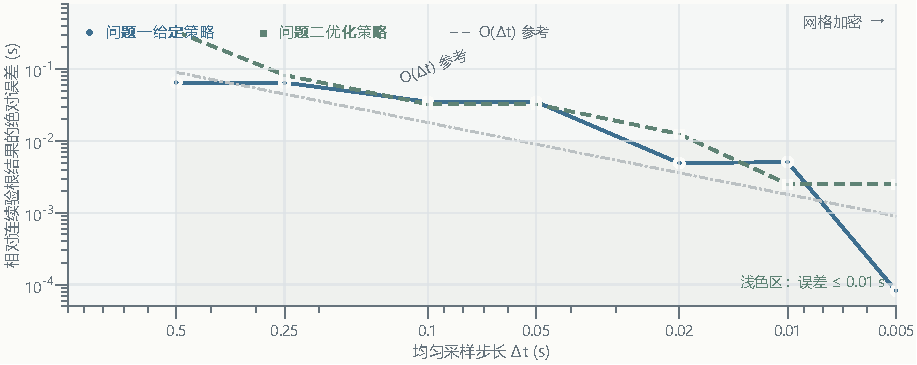
\includegraphics[width=0.90\textwidth]{time_step_convergence.pdf}
\caption{Q1、Q2 均匀计点法相对连续验根的绝对误差。横轴向右表示网格加密，虚线为 $O(\Delta t)$ 参考，浅色区标识误差不超过 $0.01$ s。}
\label{fig:time-convergence}
\end{figure}

\subsection{结果表与约束回算}

\begin{table}[H]
\centering
\caption{Q3--Q5 数值与约束审计结果}
\label{tab:numerical-audit}
\small
\begin{tabular}{lccc}
\toprule
审计项 & Q3 & Q4 & Q5\\
\midrule
结果表最大坐标重构误差/m & $3.64\times10^{-12}$ & $3.64\times10^{-12}$ & $5.46\times10^{-12}$\\
结果表最大单行时长误差/s & $9.05\times10^{-12}$ & $1.28\times10^{-12}$ & $3.24\times10^{-11}$\\
并集目标回算误差/s & $3.85\times10^{-12}$ & $5.88\times10^{-13}$ & $1.52\times10^{-11}$\\
最大约束违反量 & 0 & 0 & 0\\
\bottomrule
\end{tabular}
\end{table}

约束审计逐项检查速度上下界、同机固定航向和速度、投放时刻、引信延时、投放间隔、起爆高度以及正遮蔽时长。Q5 每架无人机相邻投放的最小间隔大于 1 s；每枚烟幕弹只写入一个导弹编号，未发生跨导弹重复计分。

\subsection{遮蔽口径敏感性}

判据敏感性对比见图\ref{fig:criterion-sensitivity}。五问的主结果与完整圆柱结果中，Q1、Q3 的相对下降分别为 $3.03\%$ 和 $1.35\%$，Q4 下降 $33.88\%$，Q5 总目标下降 $22.09\%$。Q2 两个独立终值点对应两个口径分别优化后的候选，而 Q1、Q3--Q5 是同一策略配对复算，故 Q2 不能被解释为同一决策的前后变化。

\begin{figure}[H]
\centering
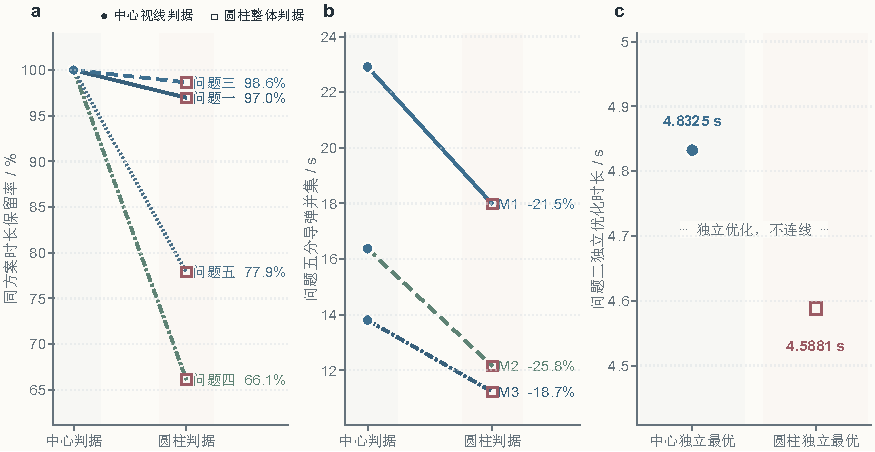
\includegraphics[width=0.98\textwidth]{criterion_sensitivity.pdf}
\caption{遮蔽判据敏感性的三层证据：跨问题同策略保留率、Q5 分导弹配对复算，以及 Q2 两种口径各自优化后的独立终值。第三部分不解释为同一策略前后损失。}
\label{fig:criterion-sensitivity}
\end{figure}

双口径比较量化的是题意几何语义的不确定性，而不是风、浓度或定位误差。本文没有这些随机量的题面数据，因此不构造虚假的分布、置信区间或 Monte Carlo 可靠度。可确认的结论是：判据改变会显著影响部分多机方案的绝对时长，完整圆柱值始终不高于对应主口径值。

\section{模型评价、适用边界与改进}

\subsection{模型特点}

本模型的运动状态由解析式给出，避免对导弹和烟幕轨迹作时间积分；有限线段投影避免把无限直线误作真实视线。连续验根与区间并集把端点精度、重叠扣除和多弹协同放在同一数学框架内。Q3--Q5 在组合前保持同机航路一致，终稿策略无需事后修补不可执行坐标。结果表回读、独立几何实现和双口径审计使主要数字能够追溯到同一次运行。

\subsection{适用边界}

\begin{enumerate}
  \item 目标中心视线是统一优化代理，不保证圆柱整体同时被遮蔽；完整圆柱审计给出更严格的同方案表现，但其方位括区也有明确的数值证据边界。
  \item 扫描后连续验根保证已括根的精度，不保证固定步长不会漏掉极窄正区间或切触。当前独立实现和步长比较降低了风险，但没有形成一般完备性证明。
  \item 球形烟幕半径、有效寿命和下沉速度均按题面硬阈值处理。若存在风和浓度衰减，球心和有效边界都会改变；当前时长不能直接外推到该场景。
  \item 导弹直线匀速且始终指向假目标。若末制导重新瞄准，导弹轨迹需替换为分段或反馈模型，后期窗口尤其可能变化。
  \item Q3--Q5 依赖有限路线库和有限状态保留。Q3/Q4 的五种子审计只刻画当前随机局部精化的离散，其中 Q3 仍明显受种子影响；Q5 的 $53.0839$ s 是固定种子下经连续复核的可行值，尚无多种子离散、全局上界或最优性间隙。
\end{enumerate}

若获得风场、定位和起爆误差的实测数据，可再建立有依据的随机轨迹与机会约束模型；在没有分布证据时，不应人为指定正态噪声。对计算方法，可用自适应区间算法同时检测符号变化和局部极值，以专门处理切触；对 Q5，可构造覆盖松弛或小规模精确子问题，用“可行值--可证明界”的间隙替代主观的最优性措辞。

\section{结论}

有限视线距离、连续事件和区间并集构成五个子问题的统一计算内核。Q1 主口径时长为 $1.4351$ s；Q2 单弹优化时长为 $4.8325$ s，8 种子连续精化结果处于双精度离散量级；Q3 三弹协同和 Q4 三机单弹协同采用各自五种子中连续复算最好的可行方案，时长分别为 $6.6311$ s 和 $15.7746$ s，其中 Q3 的种子离散明显、不能称稳定。Q5 固定种子受限路线库得到总时长 $53.0839$ s 的经验证可行解，其中 M1、M2、M3 分别为 $22.9078$、$16.3713$、$13.8049$ s；完整圆柱审计把 Q5 总时长降至 $41.3551$ s。

所有输出方案均通过连续边界、约束和结果表回算检查。最主要的模型不确定性来自遮蔽口径，最主要的算法边界来自时间括区完备性和有限路线库。本文据此只报告已验证的可行性能，不把机器精度残差当成现实鲁棒性，也不宣称 Q5 全局最优。

\section*{附录 A：复现索引}
\addcontentsline{toc}{section}{附录 A：复现索引}

\begin{table}[H]
\centering
\caption{输入、入口程序、验证文件与论文产物的对应关系}
\small
\begin{tabularx}{\textwidth}{p{2.2cm}YY}
\toprule
类别 & 文件/命令 & 用途\\
\midrule
官方输入 & \texttt{source/A题.pdf}，\texttt{source/result1--3.xlsx} & 题面、初始条件与提交字段\\
Q1--Q2 & \texttt{python -B src/solve\_q1\_q2.py} & 连续几何、单弹搜索、双口径审计\\
Q2 多种子 & \texttt{python -B src/validate\_q2\_multiseed.py} & 8 个独立种子及统计汇总\\
Q3/Q4 多种子 & \texttt{python -B src/validate\_q3\_q4\_multiseed.py} & 每问 5 个独立种子的轨迹、终值、方案与约束\\
Q3--Q5 & \texttt{python -B src/solve\_q3\_q5.py --q3-seed 20250810 --q4-seed 20250809 --q5-seed 20250808} & 路线库、候选包、有限状态搜索和连续复算\\
图件 & \texttt{python -B src/generate\_figures.py} & 从验证 JSON 生成 14 幅 PDF/PNG/SVG 图\\
验证 & \texttt{validation/q1\_independent.json}，\texttt{q1\_q2\_independent.json}，\texttt{q2\_multiseed.json}，\texttt{q3\_q4\_multiseed.json}，\texttt{q3\_q5\_independent.json} & 独立几何、连续边界、多种子、工作簿回读和约束审计\\
提交表 & \texttt{outputs/result1.xlsx}，\texttt{result2.xlsx}，\texttt{result3.xlsx} & Q3--Q5 最终可执行策略\\
\bottomrule
\end{tabularx}
\end{table}

各问种子集合、最终采用种子、求解规模、约束违反、收敛轨迹、粗评分与连续复算均保存在验证 JSON 中，并由统一运行编号 \texttt{cumcm-2025a-20260808-r3} 关联。论文数字不从聊天记录手工转录；若结果表发生修改，应重新运行坐标、区间、约束和目标回算，而不能沿用旧验证结论。

\section*{附录 B：图件主张--证据映射}
\addcontentsline{toc}{section}{附录 B：图件主张--证据映射}

\begingroup
\scriptsize
\setlength{\tabcolsep}{4pt}
\begin{longtable}{p{0.8cm}p{4.0cm}p{5.0cm}p{3.3cm}}
\caption{正文图件的唯一主张、证据源与阅读边界}\label{tab:figure-claims}\\
\toprule
图 & 唯一主张 & 数据或构造来源 & 不能推出的结论\\
\midrule
\endfirsthead
\multicolumn{4}{c}{续表\thetable}\\
\toprule
图 & 唯一主张 & 数据或构造来源 & 不能推出的结论\\
\midrule
\endhead
\bottomrule
\endlastfoot
\ref{fig:workflow} & 五问共享一条模型与验证链 & 统一模型结构 & 不证明数值正确\\
\ref{fig:sightline-geometry} & 应计算球心到有限视线段的距离 & 题面常数与解析几何 & 不指定唯一评分口径\\
\ref{fig:q1-intervals} & 两种口径的进入边界不同 & Q1 连续裕度与独立复算 & 不代表随机环境性能\\
\ref{fig:q2-surface} & Q2 截面存在零平台和狭窄高值区 & 受控二维复算 & 不是四维全局景观\\
\ref{fig:q2-multiseed} & 8 个起点经精化到同一活动面 & \texttt{q2\_multiseed.json} & 不是解析全局最优证书\\
\ref{fig:q3-union} & 多弹目标必须扣除重叠 & Q3 连续区间 & 不证明组合全局最优\\
\ref{fig:q4-synergy} & Q4 三个主窗口时间互补 & Q4 连续区间 & 不证明所有三机方案均如此\\
\ref{fig:q34-multiseed} & Q3/Q4 的局部精化与种子离散可见 & \texttt{q3\_q4\_multiseed.json} & 五种子结果不是全局最优证明\\
\ref{fig:q5-xy} & 同机策略满足共享水平航向 & Q5 结果表坐标 & 平面投影不含完整高度信息\\
\ref{fig:q5-gantt} & Q5 的逐弹区间、并集和空档可见 & Q5 连续区间 & 空档不等于可达改进量\\
\ref{fig:criterion-sensitivity} & 判据变化对各问影响不同 & Q1--Q5 验证 JSON & Q2 两柱不是同决策配对\\
\ref{fig:time-convergence} & 计点误差随分辨率变化且不宜充当报告精度 & 受控步长复算 & 不排除未被括到的切触\\
\end{longtable}
\endgroup

\begin{thebibliography}{99}
\bibitem{problem} 全国大学生数学建模竞赛组委会. 2025年高教社杯全国大学生数学建模竞赛A题：烟幕干扰弹的投放策略[EB/OL]. (2025-09-04)[2026-08-08]. \url{https://www.mcm.edu.cn/html_cn/node/03c91a444e62eee81a3740fa97a461a6.html}.
\bibitem{modelbook} 姜启源, 谢金星, 叶俊. 数学模型[M]. 5版. 北京: 高等教育出版社, 2018.
\bibitem{brent} Brent R P. Algorithms for Minimization without Derivatives[M]. Englewood Cliffs: Prentice-Hall, 1973.
\bibitem{stornprice} Storn R, Price K. Differential evolution---a simple and efficient heuristic for global optimization over continuous spaces[J]. Journal of Global Optimization, 1997, 11: 341--359.
\bibitem{powell} Powell M J D. An efficient method for finding the minimum of a function of several variables without calculating derivatives[J]. The Computer Journal, 1964, 7(2): 155--162.
\bibitem{nemhauser} Nemhauser G L, Wolsey L A. Integer and Combinatorial Optimization[M]. New York: Wiley, 1988.
\bibitem{prep} Preparata F P, Shamos M I. Computational Geometry: An Introduction[M]. New York: Springer-Verlag, 1985.
\bibitem{nocedal} Nocedal J, Wright S J. Numerical Optimization[M]. 2nd ed. New York: Springer, 2006.
\end{thebibliography}

\end{document}
